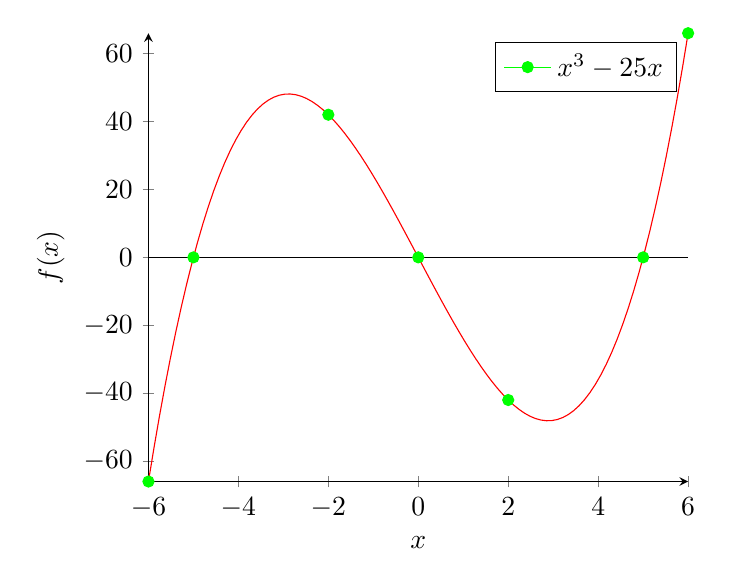
\begin{tikzpicture}
\begin{axis}[
    axis lines = left,
    xlabel = $x$,
    ylabel = {$f(x)$},
]

%Single point
\addplot[domain = -6:6, mark = *, color = green] coordinates {(0,0)};
\addplot[domain = -6:6, mark = *, color = green] coordinates {(-5,0)};
\addplot[domain = -6:6, mark = *, color = green] coordinates {(5,0)};
\addplot[domain = -6:6, mark = *, color = green] coordinates {(-2,42)};
\addplot[domain = -6:6, mark = *, color = green] coordinates {(2,-42)};
\addplot[domain = -6:6, mark = *, color = green] coordinates {(6,66)};
\addplot[domain = -6:6, mark = *, color = green] coordinates {(-6,-66)};

\addplot [
    domain=-6:6,
    samples=100,
    color=red,
]
{x^3 - 25 * x};
\addlegendentry{$x^3 - 25x$}
 \addplot [
                domain = -6:6,
                samples = 100,
                color = black,
                 ]
                {0};
\end{axis}
\end{tikzpicture}

